% debugging/debugging.tex

\QuickQuizChapter{chp:Validation}{Validation}

\section{Tracing}
\label{sec:debugging:Tracing}

\section{Assertions}
\label{sec:debugging:Assertions}

\section{Static Analysis}
\label{sec:debugging:Static Analysis}

\section{Probability and Heisenbugs}
\label{sec:analysis:Probability and Heisenbugs}

So your parallel program fails.
Sometimes.

But you figured out the problem and now have a fix in place!
Congratulations!!!

But now how much testing do you have to do in order to be certain that
you actually fixed the bug, as opposed to just reducing the probability
of it occurring on the one hand or having fixed only one of several
related bugs on the other?

Unfortunately, the honest answer is that an infinite amount of testing
is required to attain absolute certainty.

\QuickQuiz{}
	Suppose that you had a very large number of systems at your
	disposal.
	For example, at current cloud prices, you can purchase a
	huge amount of CPU time at a reasonably low cost.
	Why not use this approach to get close enough to certainty
	for all practical purposes?
\QuickQuizAnswer{
	This approach might well be a valuable addition to your
	validation arsenal.
	But it does have a few limitations:
	\begin{enumerate}
	\item	Some bugs have extremely low probabilities of occurrence,
		but nevertheless need to be fixed.
		For example, suppose that the Linux kernel's RCU
		implementation had a bug that is triggered only once
		per century of machine time on average.
		A century of CPU time is hugely expensive even on
		the cheapest cloud platforms, but we could expect
		this bug to result in more than 2,000 failures per day
		on the more than 100 million Linux instances in the
		world as of 2011.
	\item	The bug might well have zero probability of occurrence
		on your test setup, which means that you won't see it
		no matter how much machine time you burn testing it.
	\end{enumerate}
	Of course, if your code is small enough, formal validation
	may be helpful, as discussed in
	Appendix~\ref{app:formal:Formal Verification}.
} \QuickQuizEnd

But suppose that we are willing to give up absolute certainty in favor
of high probability.
Then we can bring powerful statistical tools to bear on this problem.
However, let's start with simple statistical tools.
For example, suppose that the bug had a 10\% chance of occurring in
a given run and that we do five runs.
How do we compute that probability of at least one run failing?

\begin{enumerate}
\item	Compute the probability of a given run succeeding, which is 90\%.
\item	Compute the probability of all five runs succeeding, which
	is 0.9 raised to the fifth power, or about 59\%.
\item	There are only two possibilities: either all five runs succeed,
	or at least one fails.
	Therefore, the probability of at least one failure is
	59\% taken away from 100\%, or 41\$.
\end{enumerate}

Many people find it easier to work with a formula than a series of steps,
though if you prefer the series of steps, have at it!
For those who like formulas, call the probability of a single failure $f$.
The probability of a single success is then $1-f$ and the probability
that all of $n$ tests will succeed is then:

\begin{equation}
	S_n = \left(1-f\right)^n
\end{equation}

The probability of failure is $1-S_n$, or:

\begin{equation}
	F_n = 1-\left(1-f\right)^n
\label{eq:debugging:Binomial Failure Rate}
\end{equation}

\QuickQuiz{}
	Say what???
	When I plug the earlier example of five tests each with a
	10\% failure rate into the formula, I get 59,050\% and that
	just doesn't make sense!!!
\QuickQuizAnswer{
	Remember that a probability is a number between zero and one,
	so that you need to divide a percentage by 100 to get a
	probability.
	So 10\% is a probability of 0.1, which gets a probability
	of 0.4095, which rounds to 41\%, which matches the earlier
	result.
} \QuickQuizEnd

So suppose that a given test has been failing 10\% of the time.
How many times do you have to run the test to be 99\% sure that
you have fixed the problem?

Another way to ask this question is ``how many times would we need
to run the test to cause the probability of failure to rise above 99\%?''
And if we plug $f=0.1$ into 
Equation~\ref{eq:debugging:Binomial Failure Rate} and vary $n$,
we find that 43 runs gives us a 98.92\% chance of at least one test failing
given the original 10\% per-test failure rate,
while 44 runs gives us a 99.03\% chance of at least one test failing.
So 44 runs are required for us to be 99\% certain that the failure rate
is less than 10\%.

But repeatedly plugging numbers into
Equation~\ref{eq:debugging:Binomial Failure Rate}
can get tedious, so let's solve for $n$:

\begin{eqnarray}
	F_n = 1-\left(1-f\right)^n \\
	1 - F_n = \left(1-f\right)^n \\
	log \left(1 - F_n\right) = n log \left(1 - f\right) \\
\end{eqnarray}

Finally the number of tests required is given by:

\begin{equation}
	n = \frac{1 - F_n}{1 - f}
\label{eq:debugging:Binomial Number of Tests Required}
\end{equation}

\begin{figure}[tb]
\begin{center}
\resizebox{3in}{!}{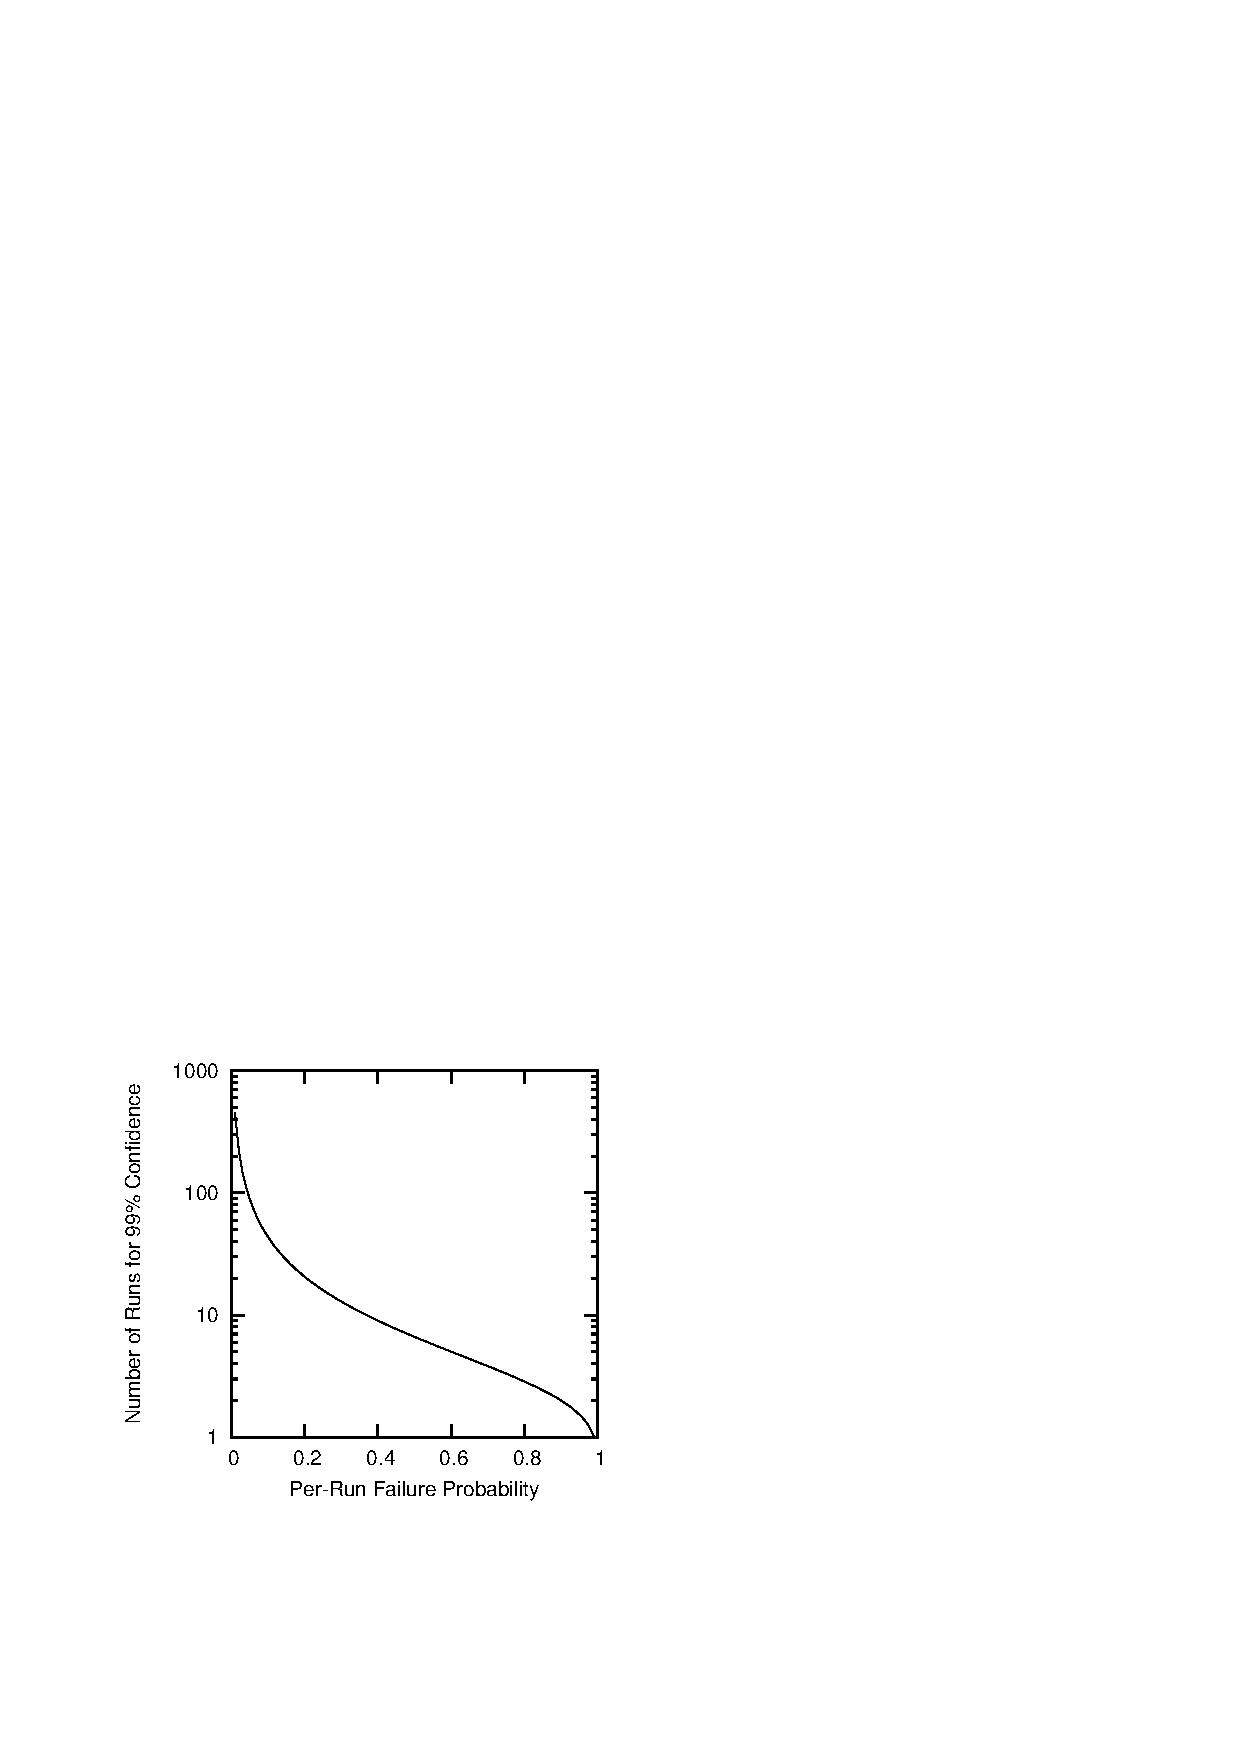
\includegraphics{CodeSamples/debugging/BinomialNRuns}}
\end{center}
\caption{Number of Tests Required for 99 Percent Confidence Given Failure Rate}
\label{fig:debugging:Number of Tests Required for 99 Percent Confidence Given Failure Rate}
\end{figure}

Figure~\ref{fig:debugging:Number of Tests Required for 99 Percent Confidence Given Failure Rate}
shows a plot of this function.
Not surprisingly, the less frequently each test run fails, the more
test runs are required to be 99\% confident that the bug has been
fixed.
If the bug caused the test to fail only 1\% of the time, then a
mind-boggling 458 test runs are required.

The moral of this story is that when you have found a rarely occurring
bug, your testing job will be much easier if you can come up with
a carefully targeted test with a much higher failure rate.
For example, if your targeted test raised the failure rate from 1\%
to 30\%, then the number of runs required for 99\% confidence
would drop from a mind-boggling 458 test runs to a mere seven test runs.

@@@ continuous formulation for time-based tests leads to Poisson distribution.

\section{Profiling}
\label{sec:analysis:Profiling}

\section{Differential Profiling}
\label{sec:analysis:Differential Profiling}

{\em @@@ pull in concepts and methods from
\url{http://www.rdrop.com/users/paulmck/scalability/paper/profiling.2002.06.04.pdf}.
Also need tools work.}

\section{Performance Estimation}
\label{sec:analysis:Performance Estimation}

{\em @@@ pull in concepts and methods from
\url{http://www.rdrop.com/users/paulmck/scalability/paper/lockperf_J_DS.2002.05.22b.pdf}.}
